\claude{
\section{Detecting simplification in neural network dynamics}\label{sec:method}
\subsection{Problem statement}
Given a scalar observation $x_t=\phi(s_t)$ of a state $s_t$, we seek changes in the complexity of its dynamics. During training, $s_t$ contains the $P$ trainable parameters and any optimizer variables. For a trained recurrent network with fixed weights, $s_t$ is its activity. These are distinct trajectories, observed through the same measurement procedure.

In a recurrent regime, let $\mu$ describe the long-run fraction of time spent in state-space regions: this is the occupation measure. We assume that this limiting measure exists and is ergodic; finite records do not prove either property. For a Euclidean ball $B(s,\epsilon)$ in a fixed state representation, define
\begin{equation}
d_{\rm act}=\lim_{\epsilon\to0^+}
\frac{\log\mu(B(s,\epsilon))}{\log\epsilon},
\label{eq:active}
\end{equation}
when the limit exists and is constant $\mu$-almost everywhere. Here $\epsilon$ is a positive radius. On a smooth manifold with positive regular density, this exponent equals the manifold dimension; $r$ independent oscillator phases therefore require $r$ local coordinates. Fixed invertible linear rescaling preserves the limit, although finite-scale estimates can change.

During nonstationary training we use a different target: a change in MG that agrees with restricted updates, reduced latent information, or more regular behavior measured independently. Such simplification need not improve performance: losing useful latent information is an undesirable change that a monitor should detect.

\subsection{Delay reconstruction and dynamical-systems theory}
A single observation can mix several components. Delayed observations can separate them by recording how the signal changes over time. We form the vector
\begin{equation}
y_t=(x_t,x_{t+\tau},\ldots,x_{t+(E-1)\tau})
\label{eq:delay}
\end{equation}
with $E$ coordinates separated by lag $\tau$. The Takens and Sauer results give conditions under which generic smooth observations distinguish the states of a deterministic system \citep{takens1981detecting,sauer1991embedology}. Extensions by Stark address forced systems under additional assumptions \citep{stark1999delay,stark2003delay}. These results explain why a scalar record can retain information about the underlying dynamics. They do not prescribe a finite-sample window or guarantee reconstruction for every SGD trajectory.

Our dimension interpretation requires the delay map to be bi-Lipschitz on the sampled support: distances may change only by bounded factors. These factors disappear in the limit in Eq.~\eqref{eq:active}, preserving local dimension. \appref{app:theory} gives the statement and proof. We test dimension recovery in recurrent systems with known structure. For applied training, we compare changes in the estimate with independent measures of simplification.

\begin{figure}[t]
\centering
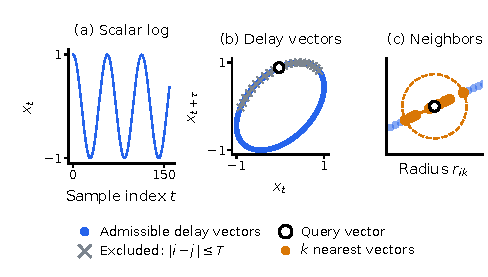
\includegraphics[width=\columnwidth]{figures/icomp_method.pdf}
\caption{\claude{Scalar samples, delay vectors, and neighbor distances. An illustrative periodic signal (a) produces the two-coordinate reconstruction (b). Panel (c) enlarges a neighborhood: blue dots are admissible vectors, gray crosses are temporally excluded, the open circle is the query, and orange dots are its $k$ nearest neighbors. The radius ratios enter Eq.~\eqref{eq:mg}.}}
\label{fig:method_geometry}
\end{figure}

\subsection{Pooled local-dimension estimation}
Within a window of $W$ scalar samples, we standardize the observations and form $n=W-(E-1)\tau$ delay vectors. For each vector, we retain $k$ nearest neighbors with time separation greater than the Theiler exclusion $T$ \citep{theiler1986spurious}. Let $r_{ij}$ be its Euclidean distance to the $j$th closest admissible neighbor, ordered increasingly. If every query has enough neighbors, we compute
\begin{equation}
\MG=\frac{n(k-1)-1}
{\displaystyle\sum_{i=1}^{n}\sum_{j=1}^{k-1}
\log(r_{ik}/r_{ij})}.
\label{eq:mg}
\end{equation}
The distance ratios measure how quickly neighborhoods fill as their radius grows; faster growth corresponds to higher local dimension. Equation~\eqref{eq:mg} pools this information across query vectors. The subtraction of one is a finite-sample correction under the local likelihood model, which assumes approximately uniform density at the neighborhood scale. Serial dependence, uneven excitation, and short records can still introduce bias. We retain these effects in the reported estimates rather than clipping values to $E$.

\paragraph{Invariance to affine rescaling.}
For fixed delay and neighbor settings, the ideal estimator is invariant to $x_t\mapsto ax_t+b$, $a\ne0$. Standardization removes the offset and amplitude scale, leaving the distance ratios unchanged. Thus MG can distinguish a change in temporal structure from a uniform change in amplitude. \appref{app:theory} proves this property and describes the effects of the small numerical noise added in the implementation. The invariance applies to a whole window; a scale change within that window can alter its temporal structure.

\paragraph{Window length and temporal resolution.}
The delay span $S=(E-1)\tau$ determines the time interval represented by each vector. The window length $W$ determines how much data enter an estimate and how precisely a transition can be located. Estimating dimension requires repeated visits within one regime. Monitoring requires a window short enough to distinguish the regimes before and after a change. We select settings on development runs and freeze them for evaluation. We also report detection delay. \appref{app:settings} lists the configurations.

\subsection{Measurement and interpretation pipeline}\label{sec:mg_conditions}
Applying the estimator requires an observable and a timescale. The following steps connect these choices to the scientific claim being tested.
\begin{enumerate}[leftmargin=*,itemsep=1pt,topsep=2pt]
\item \textbf{Choose the scalar and reference outcome.} Specify the event and an independent measurement of it. Select the observable on development runs; record at fixed intervals and measure acquisition cost.
\item \textbf{Select window, lag and decision threshold.} Before evaluation, fix the window length $W$, stride (samples between window endpoints), embedding dimension $E$, delay $\tau$, number of neighbors $k$, temporal exclusion $T$, and decision threshold. Adaptive settings need an explicit rule shared by matched runs.
\item \textbf{Compute MG and reject numerical degeneracy.} Use completed windows, dated by their endpoints. Retain raw amplitude and floor flags; check sensitivity to $W$, $\tau$, and $2E$. Report missing estimates and noise-dominated windows.
\item \textbf{Distinguish dimension recovery from change detection.} Dimension estimation requires recurrence, a stable occupation measure, a dimension-preserving observation, and sufficiently many returns above the noise scale. Otherwise, evaluate MG against the reference outcome and scalar baselines, including detection delay and false positives.
\end{enumerate}
Inadequate embedding dimension prevents faithful reconstruction, while finite-sample MG can exceed $E$. Stable estimates alone do not certify embedding assumptions; changes in SGD noise and temporal correlation can also affect the statistic.
}
